% CV template – photo & profil moved to right column
\documentclass{article}
% Encoding & core font
\usepackage[T1]{fontenc}
\usepackage[utf8]{inputenc}
\usepackage{textcomp}
\usepackage{times}
\usepackage{newtxtext} % Times‑compatible extended glyph set

% Layout
\usepackage{geometry}
\geometry{a4paper,left=0.6cm,right=0.7cm,top=1cm,bottom=1cm,columnsep=0.8cm}

% Core packages
\usepackage{fontawesome}
\usepackage[hidelinks]{hyperref}
\usepackage{multicol,paracol,tikz,adjustbox,tabularx,xcolor,enumitem}
\usepackage{ragged2e}
\newcolumntype{Y}{>{\RaggedRight\arraybackslash}X}
\setlist[itemize]{itemsep=1pt,leftmargin=*,topsep=-10pt}

% Colors
\definecolor{maincolor}{HTML}{ffffff}
\definecolor{seccolor}{HTML}{0b1f3b}
\definecolor{gray}{HTML}{8c94a9}
\definecolor{sidetext}{HTML}{59cee5}
\definecolor{Green}{HTML}{2caf00}
\definecolor{lightgray}{HTML}{D3D3D3}

% --- Side blue band ---------------------------------------------------
\usepackage{eso-pic}
\AddToShipoutPictureBG{%% background split in 70/30
  \begin{tikzpicture}[remember picture,overlay]
    \fill[seccolor] (0.7\paperwidth,0) rectangle (\paperwidth,\paperheight);
    \fill[maincolor] (0,0) rectangle (0.7\paperwidth,\paperheight);
  \end{tikzpicture}}

% ----------------------------------------------------------------------
\setlength{\parindent}{0pt}
\newcommand{\cvsection}[1]{%
  \par\bigskip
  {\bfseries\Large #1}\par
  \noindent\rule{\linewidth}{0.8pt}\par\medskip}

% Document -------------------------------------------------------------
\begin{document}\pagestyle{empty}
\columnratio{0.7}\begin{paracol}{2}

% ===================== LEFT COLUMN (70 %) =============================
{\LARGE\textbf{JUDIKAËL MOUROUVIN}}

\bigskip
{\large\textbf{Technicien support informatique \& marketing digital}}

\vspace{0.8cm}

\cvsection{EXPÉRIENCE}
\colorbox{maincolor}{%
  \begin{minipage}{\linewidth}
    \noindent
    \textbf{Alternant en marketing digital}\hfill 09/2023 - 08/2024\\
    Mairie du Gosier – DSI\\[-0.3em]
    \begin{itemize}[leftmargin=*]
      \item Analyse des besoins et déploiement de solutions numériques adaptées, améliorant l’efficacité des services. \item Support technique et formation des agents, réduisant les incidents récurrents. \item Contribution à la stratégie digitale municipale, renforçant la visibilité des projets.
    \end{itemize}
  \end{minipage}}

\vspace{3mm}

\colorbox{maincolor}{%
  \begin{minipage}{\linewidth}
    \noindent
    \textbf{Animateur de la zone informatique}\hfill 10/2022 - 08/2023\\
    Pôle emploi, Le Gosier\\[-0.3em]
    \begin{itemize}[leftmargin=*]
      \item Assistance de premier niveau auprès des demandeurs d’emploi avec un taux de satisfaction élevé. \item Configuration et maintenance des postes, limitant les interruptions de service. \item Diagnostic et résolution d’incidents matériels et logiciels, garantissant la disponibilité du parc.
    \end{itemize}
  \end{minipage}}

\vspace{3mm}

\colorbox{maincolor}{%
  \begin{minipage}{\linewidth}
    \noindent
    \textbf{Stagiaire informaticien}\hfill 09/2020 - 04/2021\\
    Numerika, Baie-Mahault\\[-0.3em]
    \begin{itemize}[leftmargin=*]
      \item Installation et entretien des équipements clients, assurant leur fiabilité. \item Support technique quotidien, réduisant les temps d’arrêt. \item Documentation des interventions pour faciliter le suivi.
    \end{itemize}
  \end{minipage}}

\cvsection{FORMATION}
\colorbox{maincolor}{%
  \begin{minipage}{\linewidth}
    \noindent
    \textbf{Bachelor Marketing digital}\hfill 09/2023 - 08/2024\\
    CFA IUTS\\[-0.3em]
    \begin{itemize}[leftmargin=*]
      \item Stratégies de communication en ligne, leviers d’acquisition. \item Conception de campagnes SEO/SEA et analyse des performances.
    \end{itemize}
  \end{minipage}}

\vspace{3mm}

\colorbox{maincolor}{%
  \begin{minipage}{\linewidth}
    \noindent
    \textbf{BTS Systèmes numériques option informatique \& réseaux}\hfill 09/2019 - 06/2021\\
    Lycée Chevalier de Saint-Georges, Les Abymes\\[-0.3em]
    \begin{itemize}[leftmargin=*]
      \item Administration systèmes et réseaux. \item Maintenance matérielle, logicielle et support utilisateur.
    \end{itemize}
  \end{minipage}}

% ===================== RIGHT COLUMN (30 %) ============================
\switchcolumn\color{white}\hspace*{0.4cm}\begin{minipage}{0.88\linewidth}

% ---- Photo -----------------------------------------------------------
\centering
\ifx\relaxc90a6ce3e5204f27853a883d0bf11c9d.png\relax\else
  \begin{tikzpicture}
    \clip (0,0) circle (1.8cm) node[anchor=center]
          {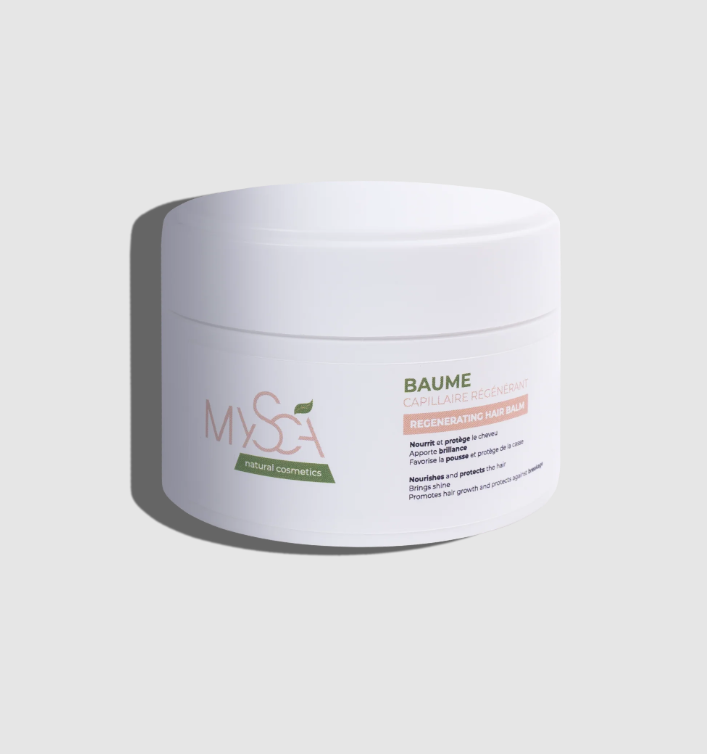
\includegraphics[width=0.2\textwidth]{c90a6ce3e5204f27853a883d0bf11c9d.png}};
  \end{tikzpicture}
\fi

% ---- Profile (Résumé) ------------------------------------------------
\cvsection{PROFIL}
\begingroup           % ouvre un groupe local
\justifying         % rétablit la justification pleine
  Passionné par l’informatique et le marketing digital, j’ai acquis une double compétence en administration systèmes/réseaux et en communication en ligne. Habitué à diagnostiquer et résoudre rapidement les incidents tout en accompagnant les utilisateurs, je sais également définir et déployer des stratégies digitales performantes. Je souhaite mettre ces atouts au service d’une organisation dynamique à temps plein.
\endgroup             % referme : on revient à \raggedright

% ---- Contact ---------------------------------------------------------
\cvsection{CONTACT}
\begin{tabular}{@{}c l}
  \faPhone & \href{tel:+590 0690 91 14 48}{+590 0690 91 14 48} \\[2pt]
  \faEnvelope & \href{mailto:jkmou971@gmail.com}{jkmou971@gmail.com} \\[2pt]
  \faMapMarker & 97190 Le Gosier \\[2pt]
  \faLinkedin & \href{}{}
\end{tabular}

% ---- Skills ----------------------------------------------------------
\cvsection{COMPÉTENCES}
\begin{itemize}[leftmargin=*]
\item Administration systèmes
\item Réseaux
\item Support utilisateur
\item Maintenance
\item Marketing digital
\item SEO / SEA
\item Configuration poste\end{itemize}

% ---- Languages -------------------------------------------------------
\cvsection{LANGUES}
\begin{itemize}[leftmargin=*]
\item English - \textcolor{gray}{}
\item Espagnol - \textcolor{gray}{}\end{itemize}

% ---- Interests -------------------------------------------------------
\cvsection{INTÉRÊTS}
\begin{itemize}[leftmargin=*]
\item Lecture
\item Sport
\item Musique
\item Voyage
\end{itemize}

\end{minipage}
\end{paracol}
\end{document}
